%!TEX root = ../thesis.tex
%*******************************************************************************
%****************************** Fourth Chapter **********************************
%*******************************************************************************
\chapter{A Web Interactive Tool for Exploring High-Dimensional Data}
\label{chapter4}

\graphicspath{{Chapter4/figs/}}

%% Cites required
One of the main focus of the state of the art proposals in Interactive ML is to provide user with the ability for hyper-parameter exploration looking to produce a good representation of embeddings and clusters. The discussion about what is a good representation, being the general problem in unsupervised learning, continues open. In addition, researchers also focus on deriving the most relevant interaction elements for supporting the data exploration. These proposals can be complemented with components for data exploration and navigation, being this a mandatory stage in any data analytics study, and model results understanding in terms of attributes in the original space.  In this work, a web interactive tool more suitable for domain-experts users with cluster-oriented tasks in high-dimensional data rather than just interaction with DR and Clustering models is presented. Design decisions about components or functionalities provided by the tool are explained in the subsequent sections. 

In addition, the decision behind implementing the tool in a web-based environment with local ML computation using only JavaScript libraries for shareability, interactivity and on-device computation is inspired by Tensorflow.js \cite{Smilkov2019TensorFlow.js:Beyond}. These properties are important for domain-expert users because enable them to perform ML-based EDA without requiring complex infrastructure and easily share their work with colleagues and community in general. By the other hand, local computation also has the advantage of privacy preserving, because despite the tool is available on internet, the data remains in the browser. Currently, the ML community in JavaScript does not have the same level of development compared to other languages like Python and R, reason why alternatives for including ML algorithms in the tool are limited. Nevertheless, it is expected that this panorama continues evolving during the next years.

\section{Data Loading}
\label{section4.1}

In many cases, domain-expert users store data in local semi-structured files, principally when the size does not demand to invest resources to maintain TI infrastructures increasing the complexity of the project.
The tool supports loading datasets from a local path in CSV format and file size constraint depends on browser capabilities. In addition, as shown in Figure \ref{fig:load-dataset-component}, 4 low size datasets for trainees are available: (1) the Fisher's Iris \cite{FisherIris}, the Zoo dataset, the Breast Cancer dataset and the Heart Diseases dataset. All these datasets are available at UCI Machine Learning Repository \cite{Dua2017UCIRepository}.

\begin{figure}[ht]
 \centering
 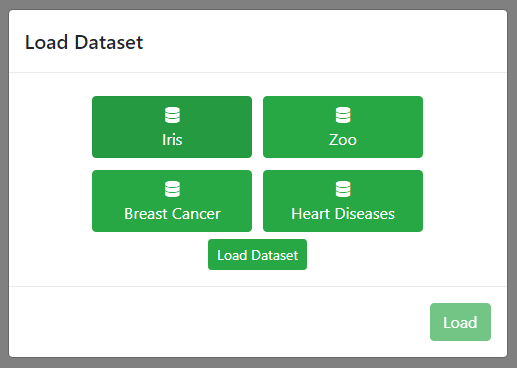
\includegraphics[width=0.5\textwidth]{load_dataset.png}
 \caption{Data Loading component.}
 \label{fig:load-dataset-component}
\end{figure}

\section{Attribute Selection}
\label{section4.2}

Attribute selection is an important stage in any ML process. After the user load a dataset, all attributes are listed including an icon representing its type and a checkbox for attribute selection. Currently, the tool is able to identify three types of attributes: numerical, boolean and categorical or strings. Boolean type is automatically identified when the attribute has only two values: 0 and 1. By default, all numerical and boolean attributes are selected meaning that these will be used for training the models. The reason behind this decision is related to the constraint of the models available in the tool of working only with numerical data. Nevertheless, categorical attributes are available for color encoding representing classes or clusters. The user can select the attribute for color encoding in the upper-right combobox, the tool automatically selects a categorical attribute with low cardinality. Figure \ref{fig:attribute-selection-component} shows the Attribute Selection component for the FIFA dataset.

\begin{figure}[ht]
 \centering
 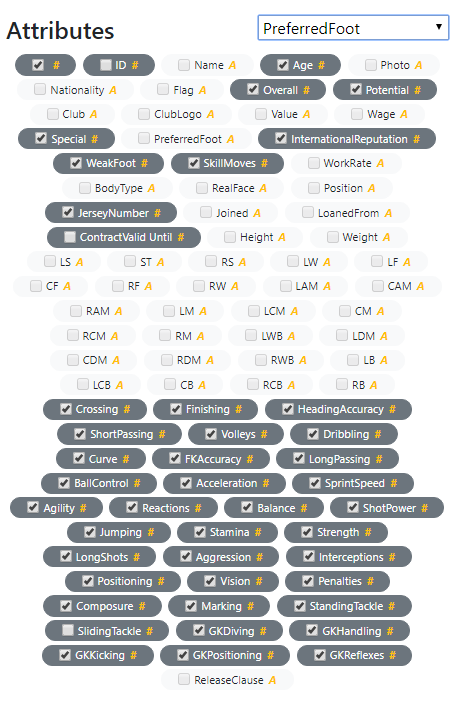
\includegraphics[width=0.5\textwidth]{attribute-selection.png}
 \caption{Attribute Selection component.}
 \label{fig:attribute-selection-component}
\end{figure}

\section{Data Exploration and Navigation (Navio)}
\label{section4.3}

The intention of using ML for exploring high-dimensional data does not imply that user should forget about descriptive techniques enabled also for gaining data understating. Distribution summarization, correlation analysis and outliers identification, among others, are generalized user tasks that always must be covered in any analytic process. Navio \cite{Guerra-Gomez2018Navio:Datasets} is an interactive web-based tool designed for achieving these kind of tasks but also for data navigation implementing three interactions: sorting, filtering a range and filtering by value. Because this tool is available as a JavaScript widget, the incorporation as a component complementary to attribute selection-level interactions looking for a more informed ML models usage is highly valuable for domain-expert users. Figure \ref{fig:navio-component} shows the Navio component for the FIFA dataset. 

\begin{figure}[ht]
 \centering
 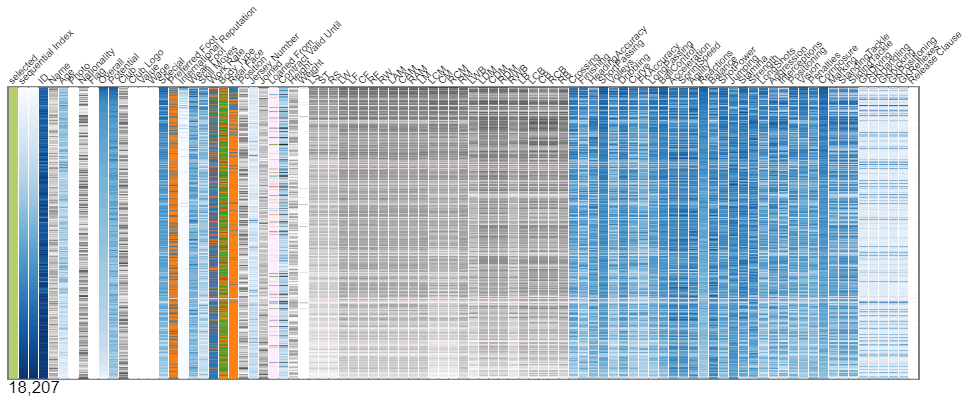
\includegraphics[width=0.9\textwidth]{navio.png}
 \caption{Data Exploration and Navigation (Navio) component.}
 \label{fig:navio-component}
\end{figure}

In addition, Navio component also includes three new attributes representing the results of the last trained models. This means, two new attributes for the embedding and other one for the clusters. In this way, user is enabled to extend the data exploration and navigation in the original space to, for instance, sort by embedding dimensions to discover correlations of them with data attributes or filter by a particular cluster. 

\section{Hyper-Parameters Exploration}
\label{section4.4}

The user is enabled to train in the browser two kind of DR and Clustering models for supporting the cluster-oriented EDA using the widely known t-SNE \cite{VanDerMaaten2008} and K-Means \cite{Lloyd1982LeastPCM} algorithms, and that currently have implementations in JavaScript \cite{Pezzotti2018LinearWeb},\cite{Asensio2018Ml-kmeans}. For both models, the user can modify the hyper-parameters in a range of values, re-train them and visualize how the embedding evolves in an iterative way. Figure \ref{fig:model-space-exploration-component} shows the Hyper-Parameter Exploration component for the FIFA dataset.

\begin{figure}[ht]
 \centering
 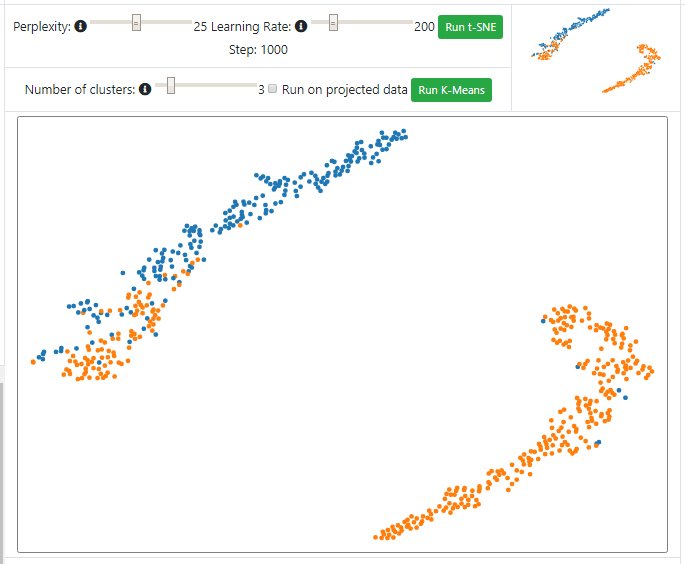
\includegraphics[width=0.7\textwidth]{model-space-exploration.png}
 \caption{Hyper-Parameter Exploration component.}
 \label{fig:model-space-exploration-component}
\end{figure}

When the training of a model finishes, additional changes to the embedding are produced: (1) Navio component is updated for including the results of the models, as explained in Section \ref{section4.3} and (2) Results Understanding component changes for evidencing the new clusters by color encoding. More details are given in Section \ref{section4.5}. In addition, the user has the option to temporally save the model results and visualize them as a mini-embedding in the upper-right component panel. This mini-embedding incorporates coordinated highlighting with the main embedding in order to compare current and previous results.

\section{Results Understanding}
\label{section4.5}

DR and Clustering models learn from similarity measures. If two data instances are close in the embedding or belongs to the same clusters, hopefully these instances will have similar attribute values. The purpose of the Results Understanding component is to evidence if this principle is fulfilled in a generalized way in order to provide trust to user and advance in the insights extraction process. For each attribute used to train the models, an idiom representing its distribution among classes and clusters is displayed. Figure \ref{fig:results-understanding-component} shows the Results Understanding component for the FIFA dataset.

\begin{figure}[ht]
 \centering
 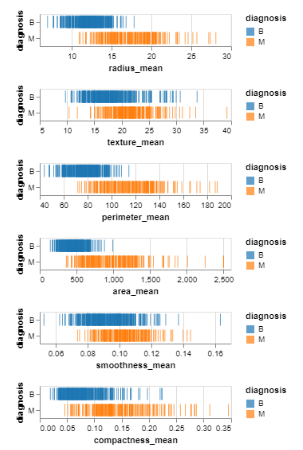
\includegraphics[width=0.5\textwidth]{results-understanding.png}
 \caption{Results Understanding component.}
 \label{fig:results-understanding-component}
\end{figure}

If user changes the attribute for color encoding in the Attribute Selection component or decide to train a new K-Means model, these idioms are automatically updated to reflect the new results. A complementary interaction element consist of a coordinated highlighting with the embedding in the Hyper-Parameter Exploration component, enabling user to obtain details on demand in two ways: highlight a set of close instances in the embedding and get their attribute values and highlight a set of instances in a range of values for one attribute and visualize how they are distributed in the embedding.

\section{Results Export}
\label{section4.6}

Finally, in any stage of the experimentation user is able to download the dataset in CSV format including three new attributes (x-axis and y-axis embedding and clusters) and a configuration file in JSON format. The downloaded dataset only includes the data instances used for training the models meaning that if user filter them using Navio, a more reduced dataset is downloaded. The configuration file contains a list of the attributes, their type and which of these were used to train the models and encode the color. Currently, this file only stores the hyper-parameters of the last trained models for the t-SNE and K-Means algorithms. Another limitation of this component is related to storing the Navio state, meaning that the interaction sequence for sorting or filtering carried out during the experimentation cannot be reproduced. In other words, user is able to observe the results of a previous experiment and re-train the models using the same hyper-parameters for achieving comparable results only if the dataset was not filtered. 